\chapter{\ifproject%
\ifenglish Project Structure and Methodology\else โครงสร้างและขั้นตอนการทำงาน\fi
\else%
\ifenglish Project Structure\else โครงสร้างของโครงงาน\fi
\fi
}

ในบทนี้จะกล่าวถึงหลักการ และการออกแบบระบบ

\section{การกำหนดแบบจำลองและทฤษฎีที่ใช้}
ในการวิจัยครั้งนี้ได้อ้างอิงทฤษฎีดุลยภาพแนช (Nash Equilibrium) และปัญหานักโทษ (Prisoner's Dilemma) เป็นกรอบแนวคิดหลัก โดยกำหนดแบบจำลองเริ่มต้นเป็นเกมที่มีผู้เล่นจำนวนสองคน คือ ผู้เล่น \(A\) และ ผู้เล่น \(B\) ซึ่งสามารถเปรียบเทียบได้กับระบบที่ประกอบด้วยสองคิวบิต (qubits) แต่ละผู้เล่นมีตัวเลือกสองทางคือ ``ยอมรับสารภาพ'' และ ``ไม่ยอมรับสารภาพ''

\subsection{ตารางผลตอบแทน (Payoff Matrix)}
ผลตอบแทนของผู้เล่นทั้งสองสามารถสรุปเป็นตารางได้ดังนี้ (รูปแบบ: \( \text{ผลตอบแทนของ A},\ \text{ผลตอบแทนของ B} \)):

\begin{table}[h]
  \centering
  \caption{Payoff matrix ของ Prisoner's Dilemma}
  \begin{tabular}{c|c|c}
    & \textbf{B: สารภาพ} & \textbf{B: ไม่สารภาพ} \\ \hline
    \textbf{A: สารภาพ}    & \(3,3\) & \(0,4\) \\ \hline
    \textbf{A: ไม่สารภาพ} & \(4,0\) & \(1,1\)
  \end{tabular}
\end{table}

\section{การสร้างแบบจำลองเบื้องต้นเพื่อนำมาประยุกต์ใช้}
กำหนดให้
\[
X \equiv \text{ผู้เล่น A},\qquad Y \equiv \text{ผู้เล่น B}
\]
โดยทั้ง \(X\) และ \(Y\) มีค่าได้เพียงสองสถานะเท่านั้น คือ
\[
0 = \text{ไม่รับสารภาพ},\qquad 1 = \text{ยอมรับสารภาพ}.
\]

\subsection{เหตุการณ์ที่ 1: ผู้เล่น A พ้นโทษ}
\[
\begin{aligned}
x=0,\ y=0 &\longrightarrow f(0,0)=1,\\
x=0,\ y=1 &\longrightarrow f(0,1)=4,\\
x=1,\ y=0 &\longrightarrow f(1,0)=0,\\
x=1,\ y=1 &\longrightarrow f(1,1)=3.
\end{aligned}
\]
และฟังก์ชันผลตอบแทนรวมพร้อมบทลงโทษ:
\[
g(x,y) = f(x,y) + \alpha(1-x) + \beta y, \quad \alpha=\beta=1
\]
คำนวณค่าต่าง ๆ ได้เป็น
\[
\begin{array}{l|cc}
(x,y) & f(x,y) & g(x,y) \\ \hline
(0,0) & 1 & 2\\
(0,1) & 4 & 6\\
(1,0) & 0 & 0\\
(1,1) & 3 & 4
\end{array}
\]

\subsection{เหตุการณ์ที่ 2: B ติดคุกน้อยที่สุด}
\[
f(x,y) = 1(1-x)(1-y) + 0(1-x)y + 4x(1-y) + 3xy
\]
\[
g(x,y) = 1 + \beta + (3+\alpha)x - (1+\beta)y, \quad \alpha=\beta=1
\]
\[
\begin{array}{l|cc}
(x,y) & f(x,y) & g(x,y) \\ \hline
(0,0) & 1 & 2\\
(0,1) & 0 & 0\\
(1,0) & 4 & 6\\
(1,1) & 3 & 4
\end{array}
\]

\subsection{เหตุการณ์ที่ 3: ทั้งคู่ไม่รับสารภาพ}
\[
f(x,y) = 2(1-x)(1-y) + 4(1-x)y + 4x(1-y) + 6xy
\]
\[
g(x,y) = (2+\alpha)x - (2+\alpha)y + 2, \quad \alpha=\beta=1
\]
\[
\begin{array}{l|cc}
(x,y) & f(x,y) & g(x,y) \\ \hline
(0,0) & 2 & 2\\
(0,1) & 4 & 5\\
(1,0) & 4 & 5\\
(1,1) & 6 & 8
\end{array}
\]

\subsection{เหตุการณ์ที่ 4: ทั้งคู่ยอมรับสารภาพ}
\[
g(x,y) = (3x-3)^2 + (3y-3)^2
\]
\[
\begin{array}{l|c}
(x,y) & g(x,y) \\ \hline
(0,0) & 18\\
(0,1) & 9\\
(1,0) & 9\\
(1,1) & 0
\end{array}
\]

\section{การตรวจสอบความถูกต้องผ่านการประมวลผลด้วยไลบรารีควอนตัม}
  

  \begin{figure}
  \begin{center}
  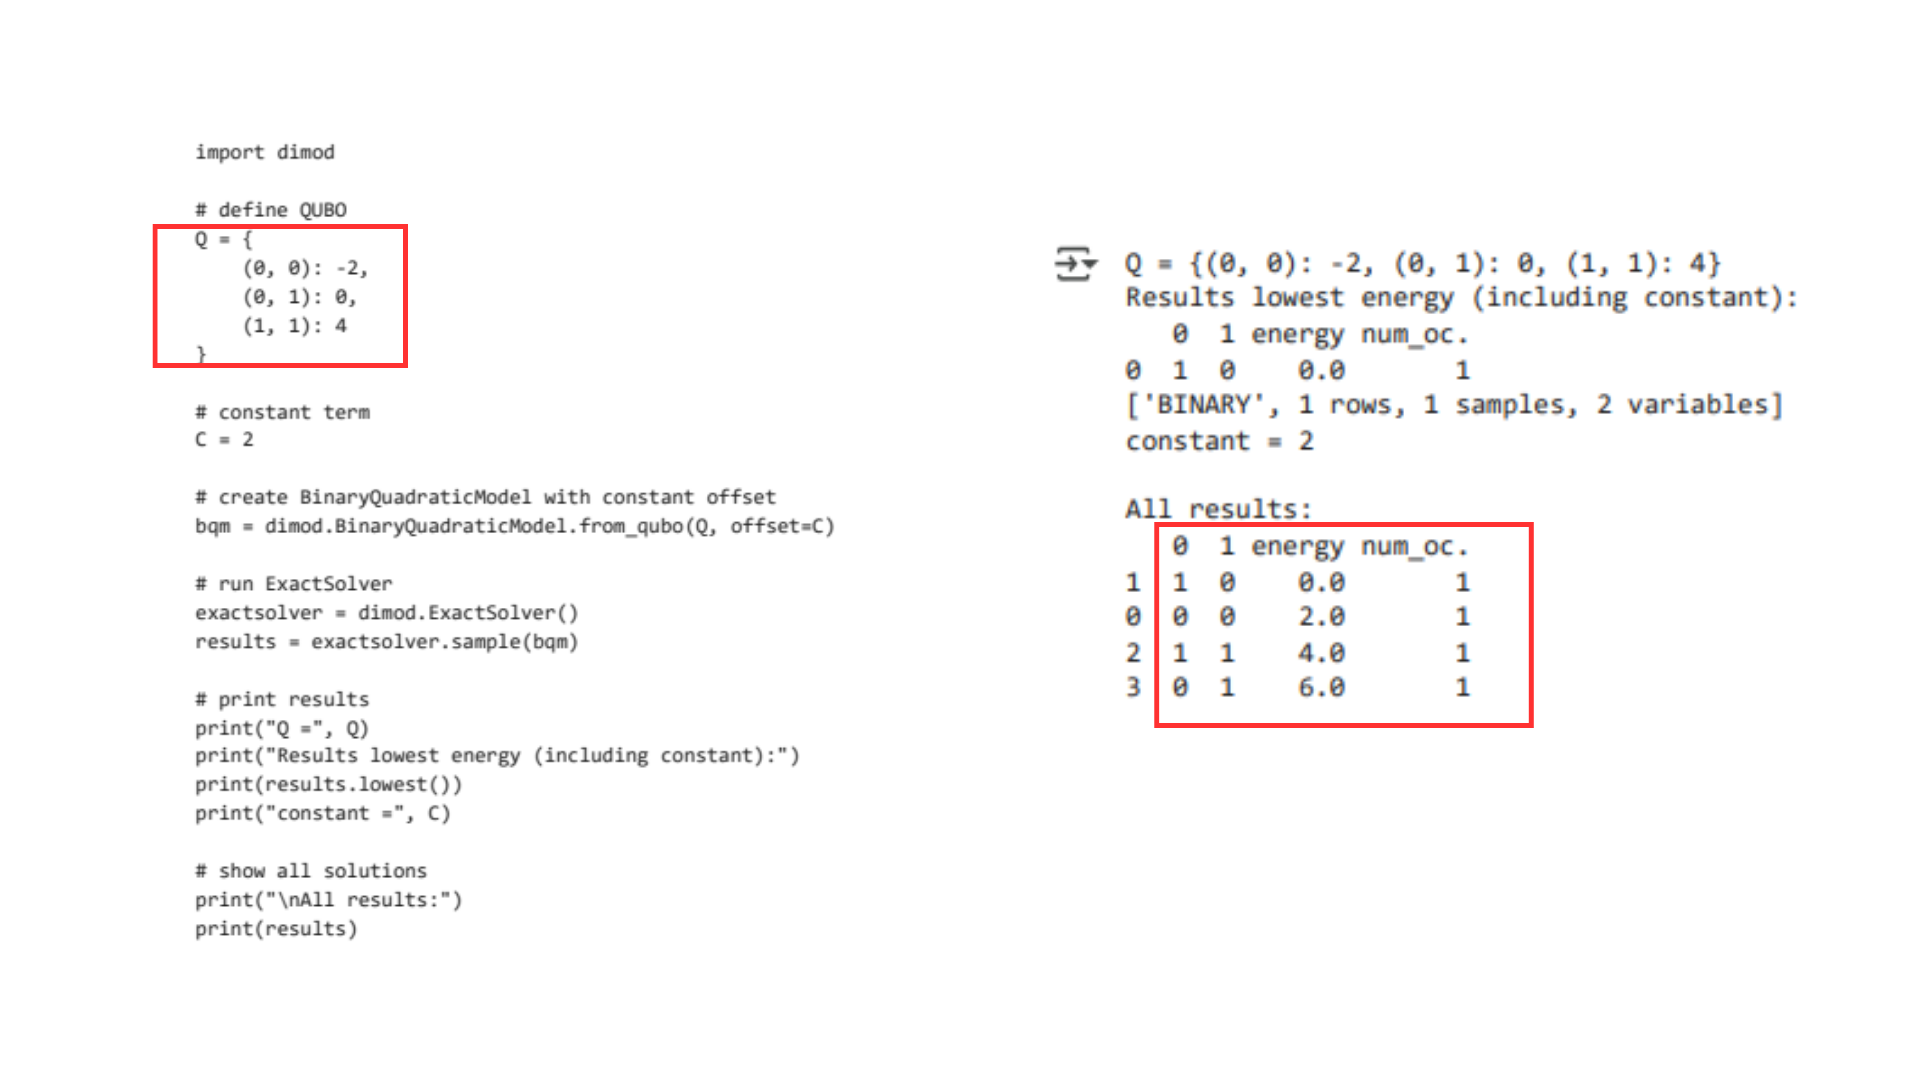
\includegraphics[width=5.5in]{case1_RunPicture.png}
  \end{center}
  \caption[Poem]{ภาพผลลัพธ์เหตุการณ์ที่ 1 หลังจากประมวลผลผ่านไลบรารีควอนตัม }
  \end{figure}

  \begin{figure}
    \begin{center}
    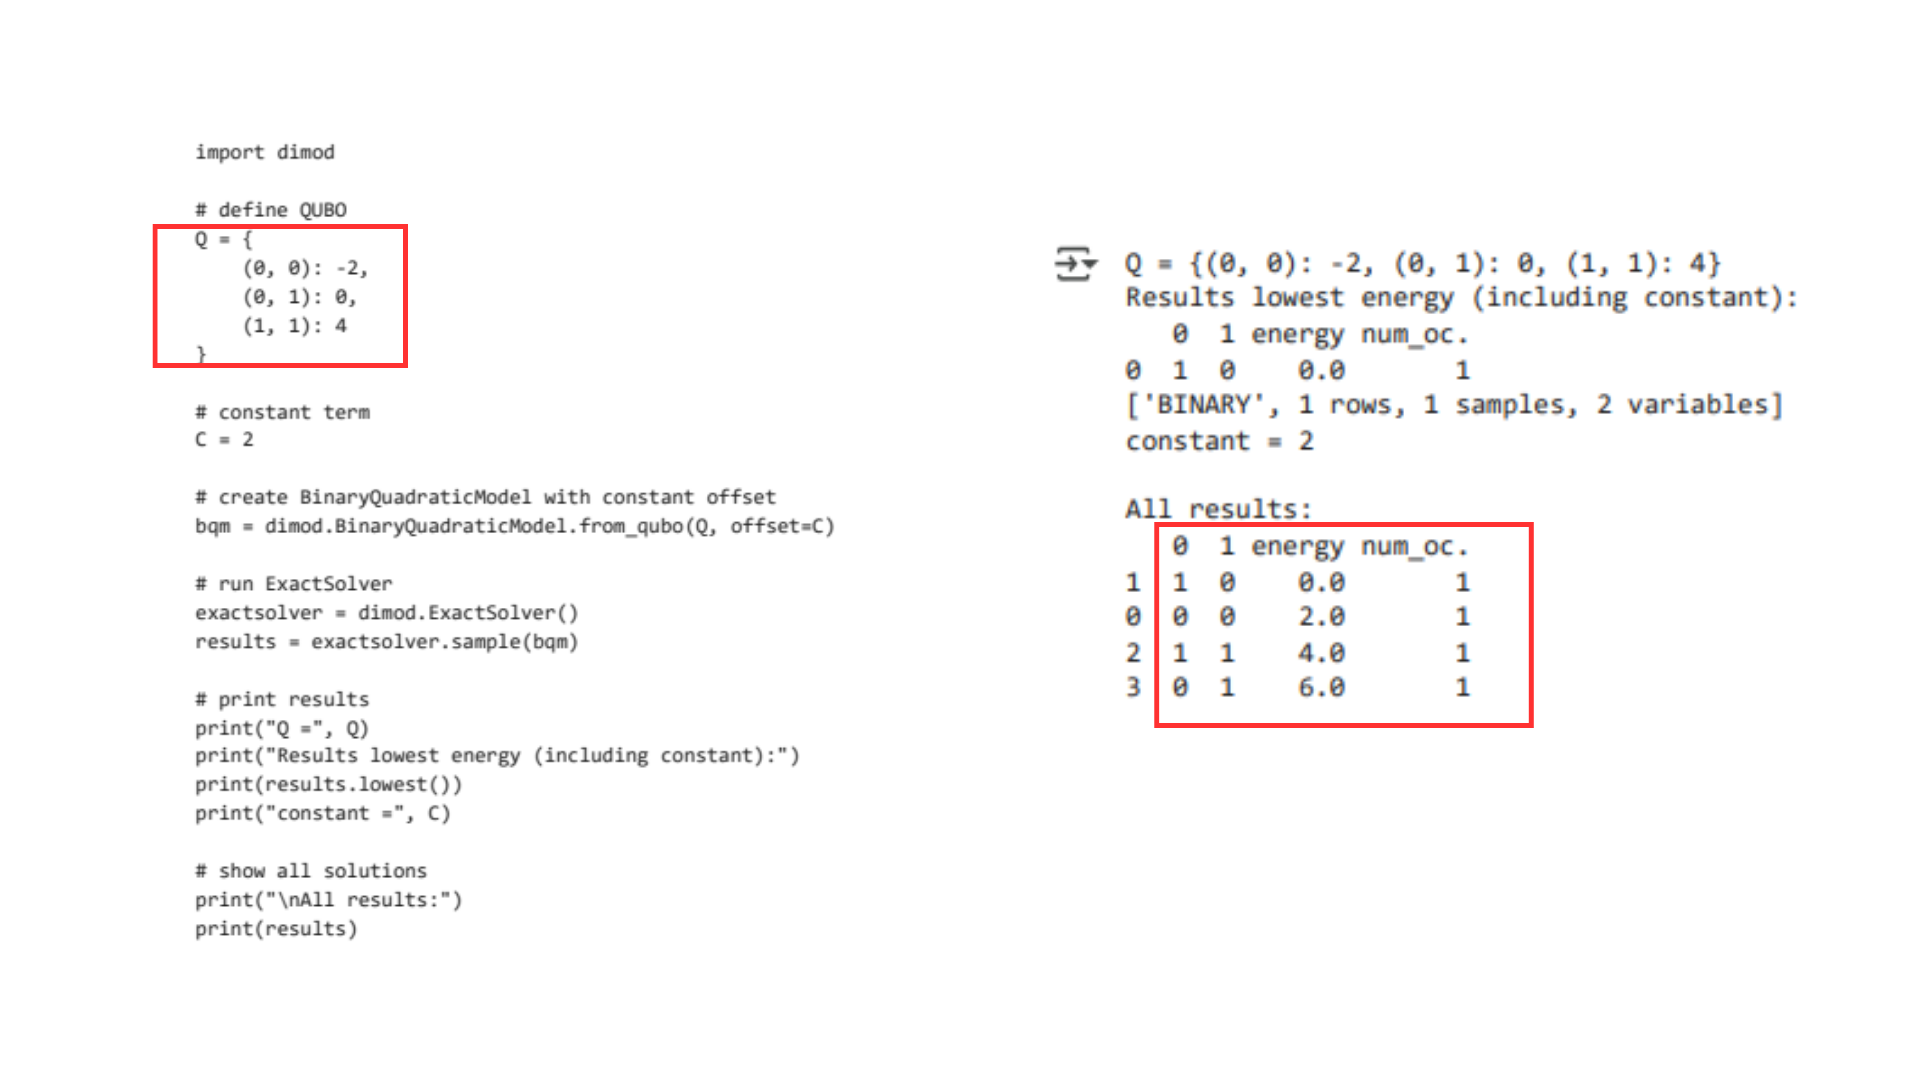
\includegraphics[width=5.5in]{case1_RunPicture.png}
    \end{center}
    \caption[Poem]{ภาพผลลัพธ์เหตุการณ์ที่ 1 หลังจากประมวลผลผ่านไลบรารีควอนตัม }
    \end{figure}

    \begin{figure}
      \begin{center}
      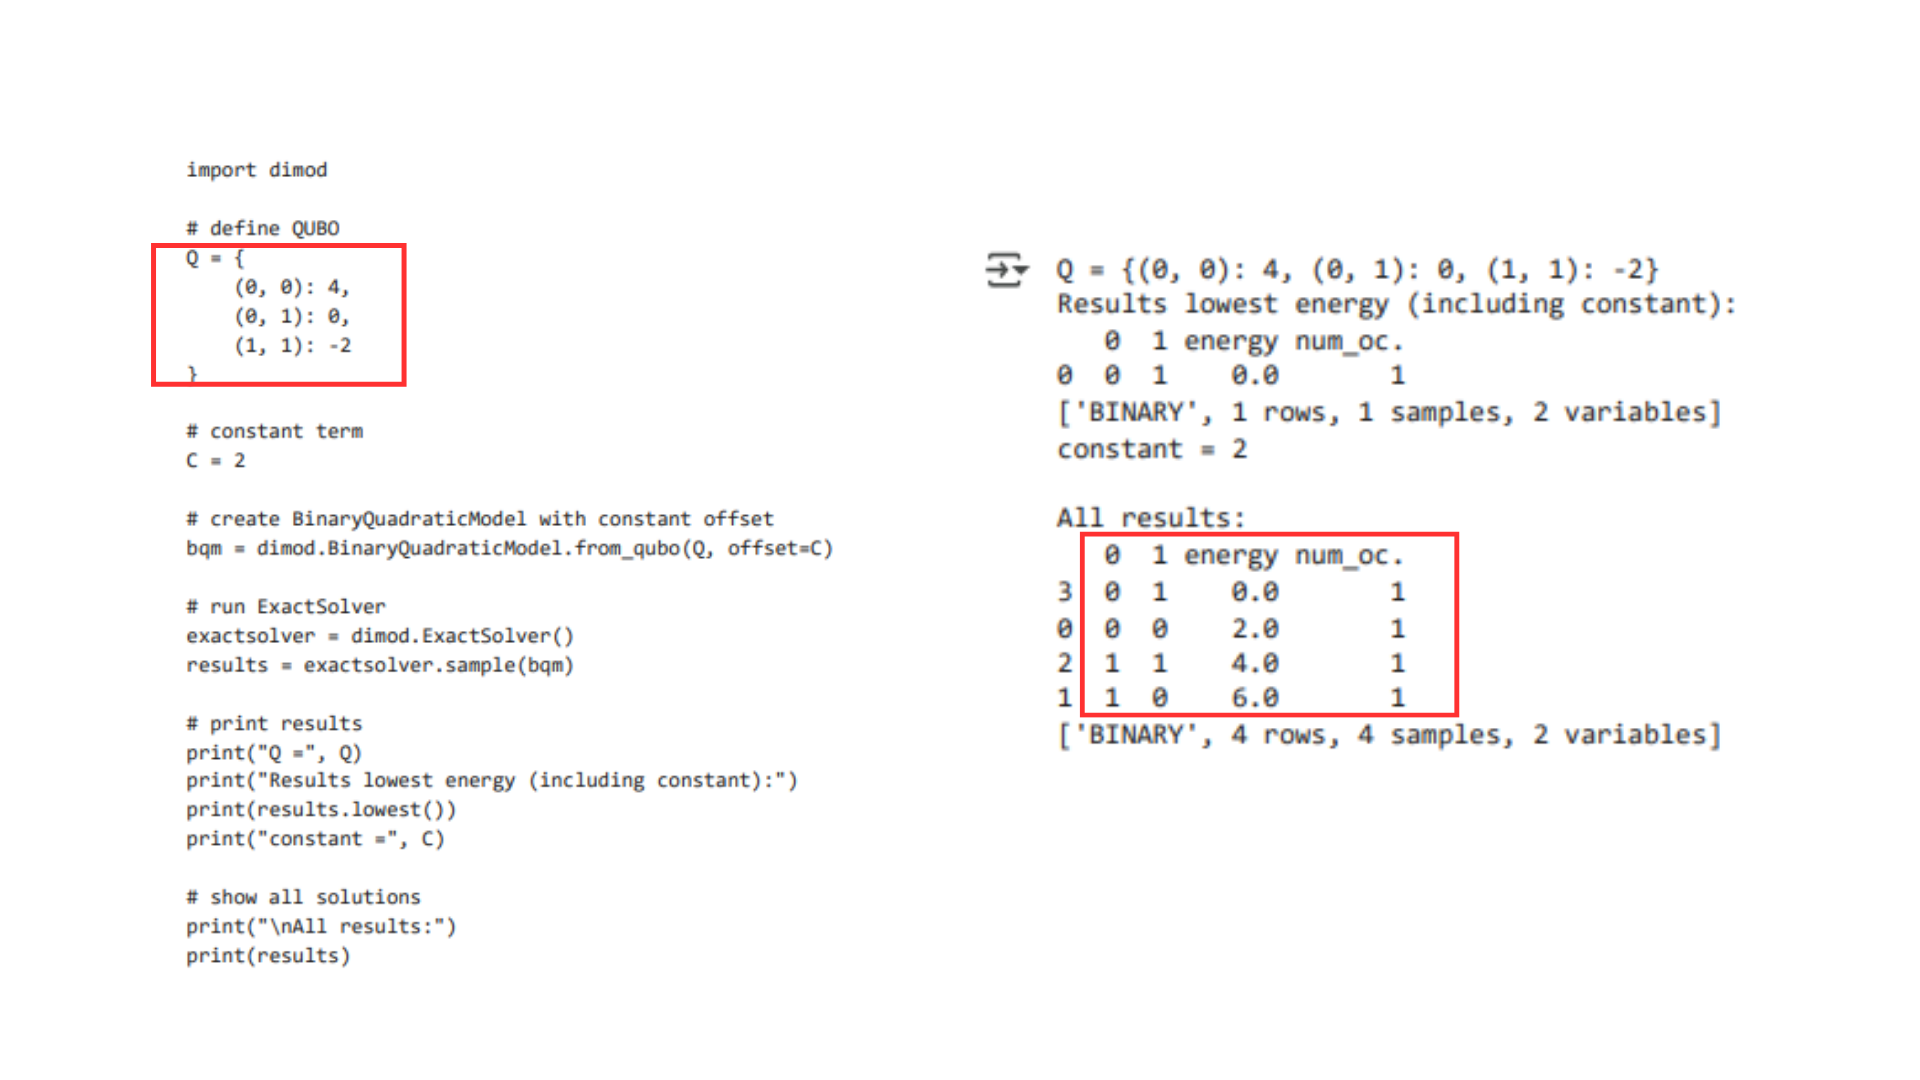
\includegraphics[width=5.5in]{case2_RunPicture.png}
      \end{center}
      \caption[Poem]{ภาพผลลัพธ์เหตุการณ์ที่ 2 หลังจากประมวลผลผ่านไลบรารีควอนตัม }
      \end{figure}
      \begin{figure}
        \begin{center}
        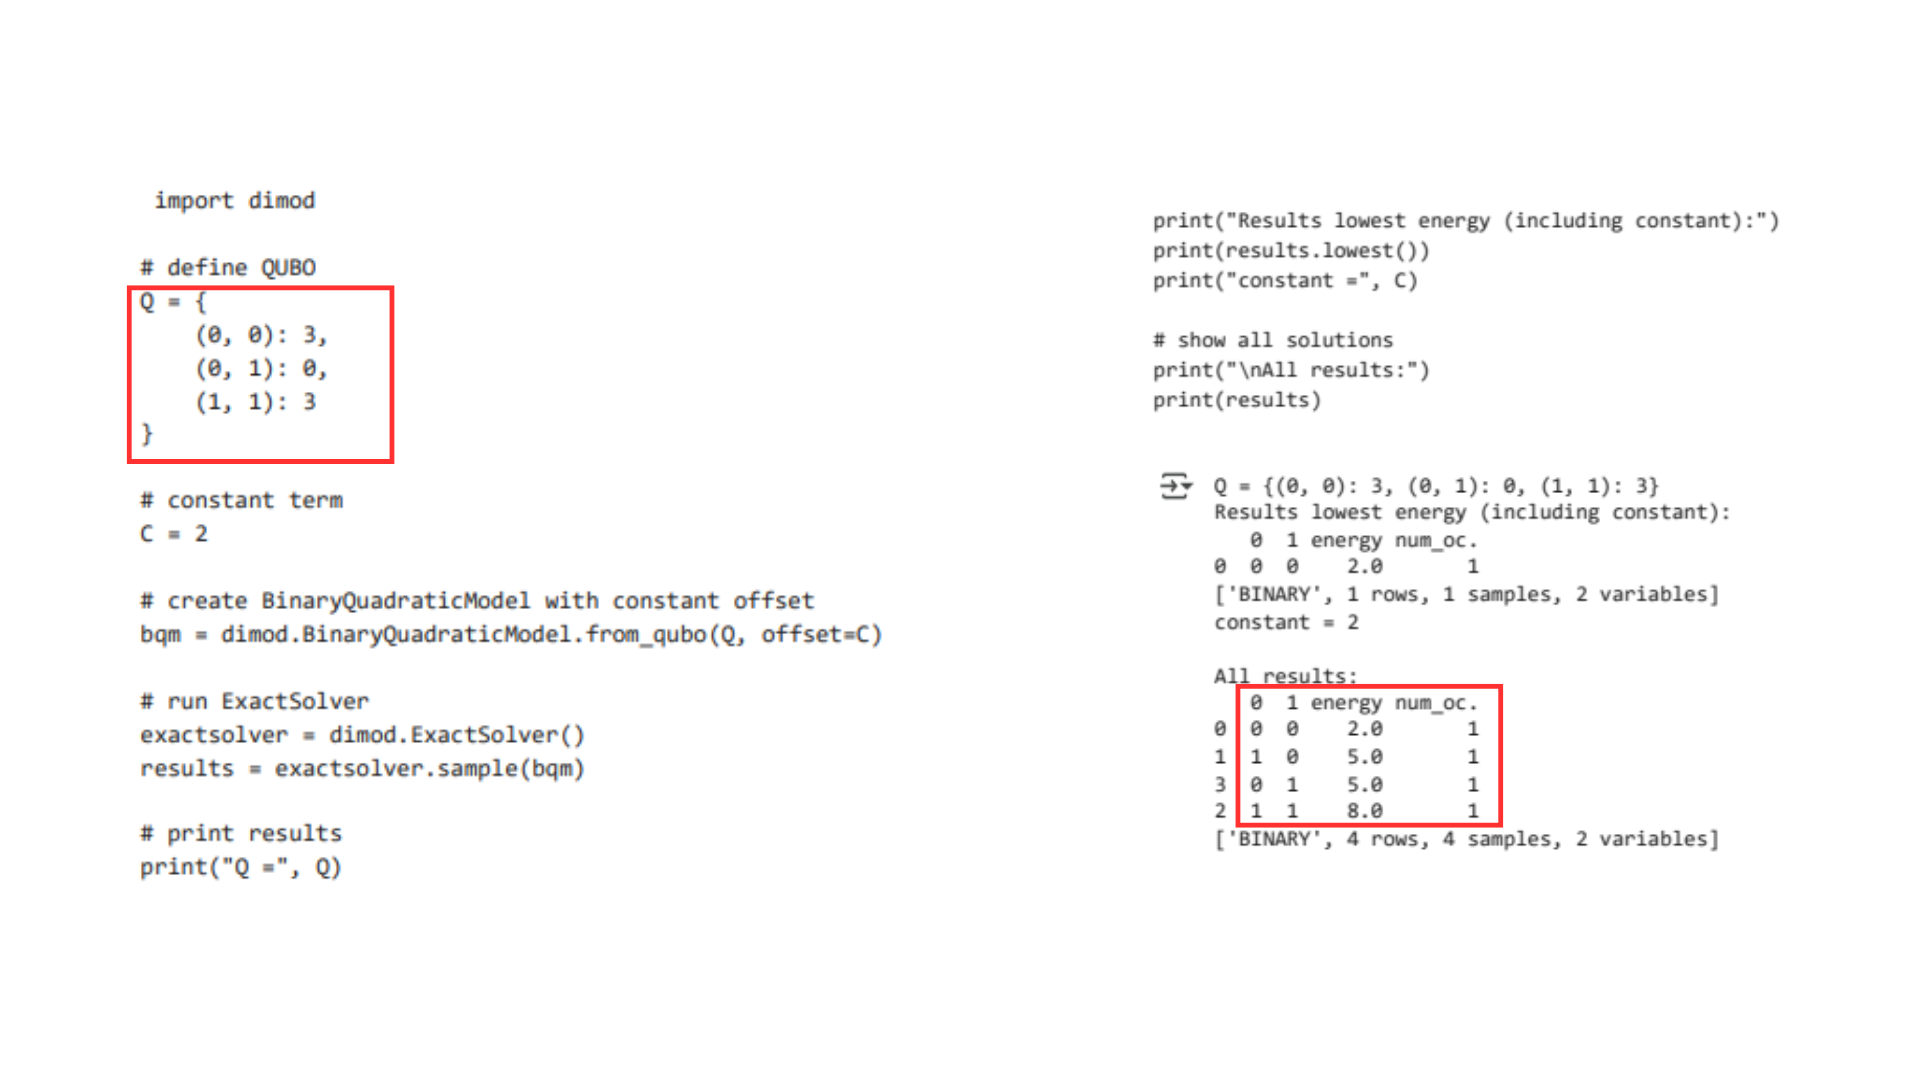
\includegraphics[width=5.5in]{case3_RunPicture.png}
        \end{center}
        \caption[Poem]{ภาพผลลัพธ์เหตุการณ์ที่ 3 หลังจากประมวลผลผ่านไลบรารีควอนตัม }
        \end{figure}

        \begin{figure}
          \begin{center}
          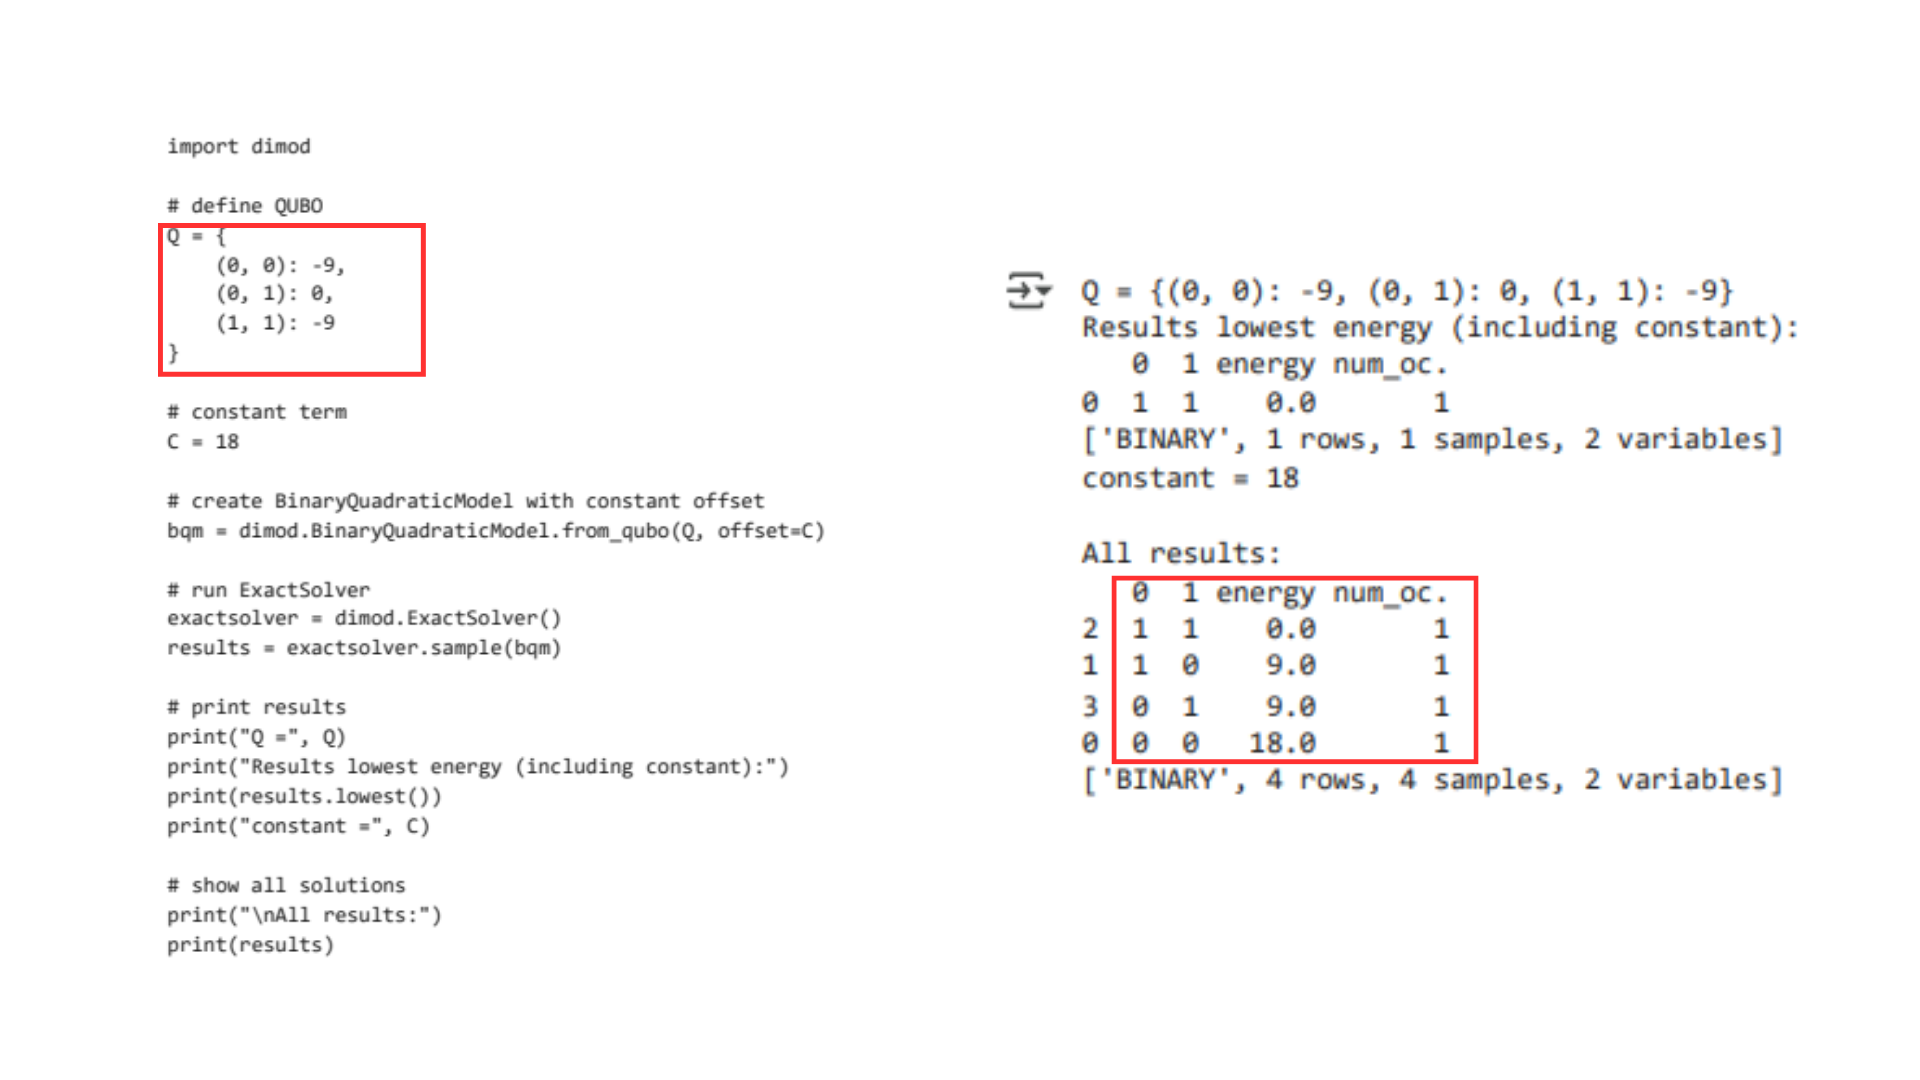
\includegraphics[width=5.5in]{case4_RunPicture.png}
          \end{center}
          \caption[Poem]{ภาพผลลัพธ์เหตุการณ์ที่ 4 หลังจากประมวลผลผ่านไลบรารีควอนตัม }
          \end{figure}
  

\section{การประยุกต์ข้อมูลทางไซเบอร์เพื่อสร้างแบบจำลองการโจมตีและป้องกัน}
ในการศึกษานี้ได้ประยุกต์ใช้ข้อมูลเชิงไซเบอร์ (cyber data) เพื่อสร้างแบบจำลอง (model) ที่วิเคราะห์ผลกระทบจากการโจมตี (damage) และผลประโยชน์จากการป้องกัน (benefit) โดยใช้โครงสร้างข้อมูลแบบต้นไม้ (Tree Structure)

\begin{itemize}
  \item \textbf{โหนด (Nodes):} แทนทรัพย์สินหรือสินทรัพย์สารสนเทศ (Asset Value / Payoff Asset Value)
  \item \textbf{เส้นเชื่อม (Edges):} แทนต้นทุนในการป้องกัน (Defense Cost)
\end{itemize}

ผู้โจมตี (attacker) ต้องเลือกเส้นทาง (path) ผ่านโครงสร้างต้นไม้โดยคำนึงถึงงบประมาณ ขณะที่ผู้ป้องกัน (defender) ต้องจัดกลยุทธ์เพื่อปกป้องโหนดที่สำคัญที่สุด
\section{วิธีการและแนวทางเชิงอัลกอริทึม}

เพื่อให้สามารถหากลยุทธ์การโจมตีและป้องกันที่เหมาะสมได้ มีการใช้แนวคิดทางอัลกอริทึมดังนี้

\subsection{Depth-First Search (DFS)}
ใช้สำรวจเส้นทางจากรากต้นไม้ (root node) ไปยังใบ (leaf node) โดยพิจารณาทุกเส้นทางอย่างละเอียด เพื่อค้นหาความเป็นไปได้ของการโจมตีและการป้องกันในกรณีต่าง ๆ เหมาะสำหรับการตรวจสอบเส้นทางเฉพาะเจาะจงและหา path ที่มี payoff สูงหรือมีต้นทุนต่ำ

\subsection{Breadth-First Search (BFS)}
ใช้สำรวจเชิงกว้าง (layer-by-layer) เพื่อประเมินความเสี่ยงในระดับชั้น (layers) ของต้นไม้ ทำให้สามารถระบุได้ว่าในระดับใดของโครงสร้างมีจุดอ่อนหรือมีโหนดที่มีความสำคัญสูงต่อระบบ เหมาะสำหรับการวิเคราะห์ระดับความลึกและการค้นหาช่องโหว่ที่อยู่ใกล้ราก

\subsection{Greedy Algorithm}
ใช้หลักการเลือกโหนดที่มีค่ารางวัล (payoff / asset value) สูงที่สุดก่อน สร้างกลยุทธ์การป้องกันแบบ ``Most Prizes First'' ช่วยให้ผู้ป้องกันสามารถจัดสรรทรัพยากรที่มีอยู่อย่างจำกัดได้อย่างมีประสิทธิภาพ โดยอาจผสานกับข้อจำกัดงบประมาณ (budget-aware) เพื่อเลือกชุดโหนดที่ให้ผลตอบแทนสุทธิดีที่สุด

\section{แนวทางการป้องกัน (Defense Strategy)}

ผู้ป้องกันสามารถใช้กลยุทธ์ดังต่อไปนี้:

\subsection{Most Prizes First}
จัดสรรทรัพยากรไปยังโหนดที่มีค่ารางวัล (payoff / asset value) สูงที่สุดก่อน เพื่อให้การป้องกันมีประสิทธิภาพสูงสุด

\subsection{Budget-Aware Defense}
พิจารณาการป้องกันภายใต้งบประมาณที่จำกัด โดยเลือกชุดโหนด (combination) ที่ทำให้ผู้โจมตีไม่สามารถได้ผลตอบแทนเกินระดับที่กำหนด

\subsection{Hybrid DFS + Greedy}
ใช้ DFS สำรวจเส้นทางที่เป็นไปได้ทั้งหมดร่วมกับ Greedy Algorithm เพื่อเลือกป้องกันโหนดที่มี payoff สูงสุด

\section{การตรวจสอบ พัฒนา และประมวลผล (เนื้อหา 261492)}


\section{การสร้างแผนภาพและการรายงานผล(เนื้อหา 261492)}

